\documentclass{standalone}
\usepackage{graphicx}	
\usepackage{amssymb, amsmath}
\usepackage{color}

\usepackage{tikz}
\usetikzlibrary{intersections, backgrounds}

\definecolor{light}{RGB}{220, 188, 188}
\definecolor{mid}{RGB}{185, 124, 124}
\definecolor{dark}{RGB}{143, 39, 39}
\definecolor{highlight}{RGB}{180, 31, 180}
\definecolor{gray10}{gray}{0.1}
\definecolor{gray20}{gray}{0.2}
\definecolor{gray30}{gray}{0.3}
\definecolor{gray40}{gray}{0.4}
\definecolor{gray60}{gray}{0.6}
\definecolor{gray70}{gray}{0.7}
\definecolor{gray80}{gray}{0.8}
\definecolor{gray90}{gray}{0.9}
\definecolor{gray95}{gray}{0.95}

\newcommand*{\offset}{0.025}

\begin{document}

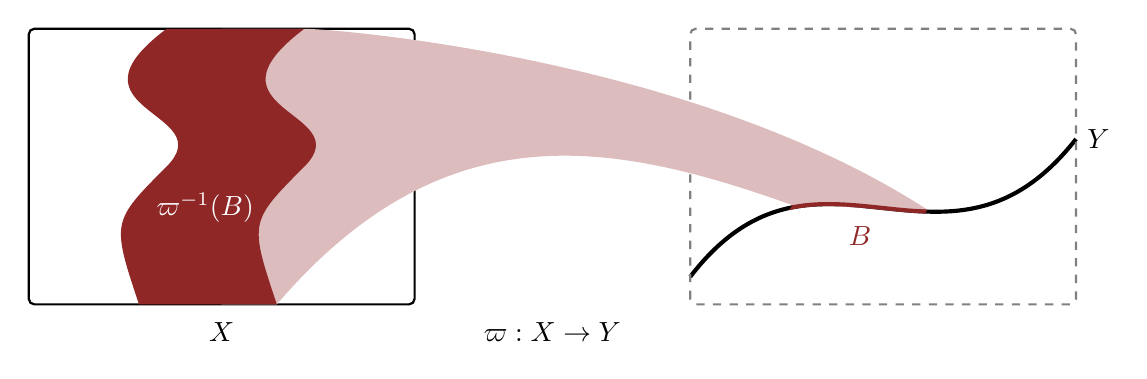
\begin{tikzpicture}[scale=0.35, thick]
  \draw [rounded corners=2pt, color=black] (-5, 0) rectangle +(-14, 10);
  \node at (-12, -1) { $X$ };
  \node at (0, -1) { $\varpi: X \rightarrow Y$ };
  
  \draw [line width=1.5] (5, 1) .. controls (9.6, 7) and (14.3, 0) .. (19, 6)
  node[right] { $Y$ };
  
  \draw [rounded corners=2pt, color=gray, dashed] (5, 0) rectangle +(14, 10);
  
  \fill [color=light] (-12, 10) -- (-9, 10) .. controls (-8, 10) and (5, 9) .. (13.6, 3.44) 
                       -- (8.71, 3.6) .. controls (2, 6) and (-4, 7) .. (-10, 0) -- (-12, 0);

  %\draw [color=green] (-14, 4.9) circle (0.15);
  %\draw [color=green] (13.6, 3.35) circle (0.15);
  %\draw [color=green] (8.71, 3.53) circle (0.15);
  %\draw [color=green] (-11.2, 2.1) circle (0.15);
                     
  \begin{scope}
    \clip (9, 0) .. controls (8, 3) .. (10, 5) ..
          controls (12, 7) and (6, 7) .. (10, 10)
          -- (15, 10) .. controls (11, 7) and (17, 7) 
          .. (15, 5) .. controls (13, 3) .. (14, 0)
          -- cycle; 
    \draw [color=dark, line width=1.5] (5, 1) .. controls (9.6, 7) and (14.3, 0) .. (19, 6)
    node[midway, xshift=-8, yshift=-10] { $B$ };
  \end{scope}
  
  \fill [color=dark] (-10, 0) .. controls +(-1, 3) .. +(1, 5) .. 
                              controls +(2, 2) and +(-4, -3) .. +(1, 10) 
                              -- (-14, 10) .. controls +(-4, -3) and +(2, 2) 
                              .. +(0, -5) .. controls +(-2, -2) .. +(-1, -10) -- (-10, 0);
  
  \fill [dark, text=white] (-12.6, 3.5) circle (2)
  node {$\varpi^{-1}(B)$};
  
  %\fill [green, text=white] plot [smooth cycle, tension=1] coordinates 
  %      {(-15.6, 3) (-13, 5.5) (-9.5, 6.25) (-10.4, 3.5) (-12.5, 3.5) (-14, 2)};
  
\end{tikzpicture}

\end{document}  